\subsection{テストプロセス}
テスト技法や測度は、定義されたテストプロセスに組み込まれて初めて実務で機能する。テストプロセスは、組織レベル、管理レベル、動的テストレベルの多層構造で考えられる。組織レベルでは方針や戦略を作る。管理レベルでは計画、監視、制御、完了を扱う。動的テストレベルでは設計、実装、環境構築、実行、インシデント報告を扱う。

\begin{figure}[htbp]
\centering
\IfFileExists{assets/generated_figures/ch05/fig-ch05-12.png}{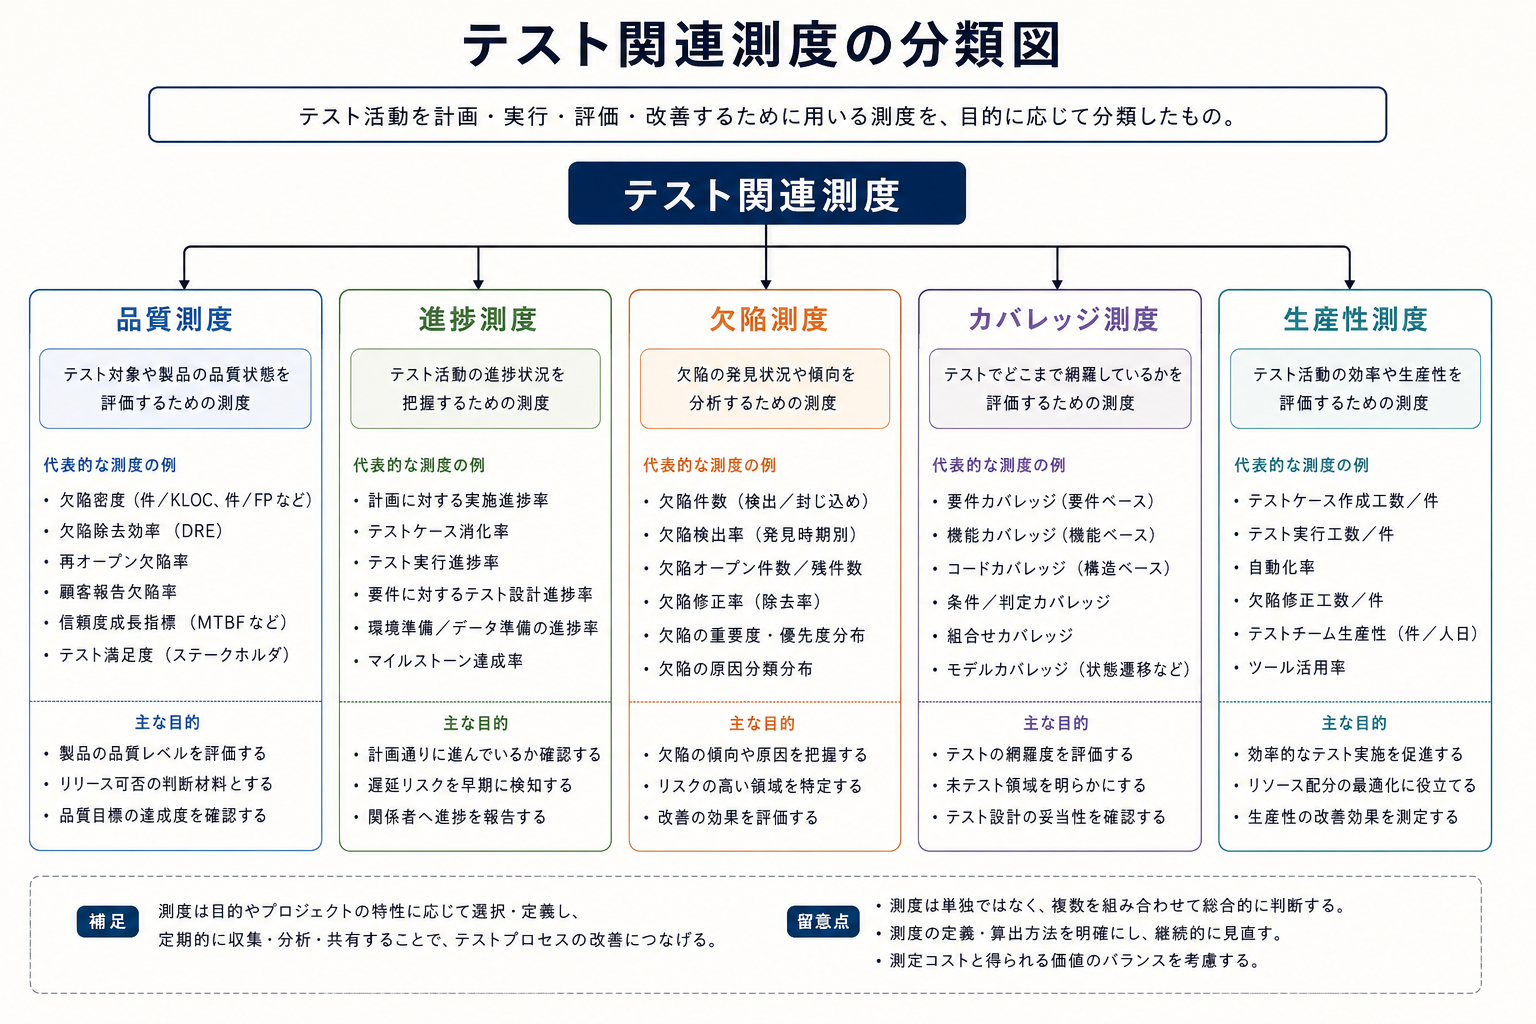
\includegraphics[width=0.96\linewidth]{assets/generated_figures/ch05/fig-ch05-12.png}}{\fbox{\parbox[c][48mm][c]{0.9\linewidth}{\centering 画像生成待ち\\テストプロセスの多層図}}}
\caption{テストプロセスの多層図}
\label{fig:ch05-12}
\end{figure}

\subsubsection{実務上の考慮}
\paragraph{態度とエゴレスプログラミング}
テストで重要なのは、障害発見を個人攻撃と見なさない態度である。欠陥が見つかることは、品質を改善する機会である。管理者は、失敗の発見と修正を歓迎する文化を作る必要がある。アジャイルやシフトレフトでは、テスターと開発者の協調が成功に不可欠である。

\paragraph{テスト指針と組織プロセス}
組織は、テスト方針とテスト戦略を定義する。テスト方針は、テストの目的、目標、全体範囲を示す。テスト戦略は、どのようにテストするかの指針である。リスクベーステストでは、製品リスクをもとにテストの焦点と優先度を決める。

\paragraph{テスト管理と動的テストプロセス}
テスト管理には、計画、監視、制御、完了が含まれる。動的テストプロセスには、テスト設計と実装、テスト環境の準備と保守、テスト実行、インシデント報告が含まれる。これらは、人、ツール、方針、測度を組み合わせてライフサイクルに統合される。

\paragraph{テスト文書化}
テスト文書は、組織テスト文書、テスト管理文書、動的テスト文書に分けられる。組織テスト文書には方針や戦略が含まれる。テスト管理文書にはテスト計画、状況報告、完了報告が含まれる。動的テスト文書にはテスト設計仕様、テストケース仕様、手順仕様、データ要求、環境要求、実行ログ、インシデント報告などが含まれる。

\paragraph{テストチーム}
テストチームの構成は、費用、納期、組織成熟度、アプリケーションの重要度によって変わる。開発者自身がテストする場合も、独立したテスト担当者が行う場合もある。シフトレフトでは、開発者、テスター、顧客が早い段階から協力し、役割の境界が薄くなることがある。

\paragraph{テストプロセス測度}
テストプロセスでは、指定済み、実行済み、合格、不合格のテストケース数、未解決欠陥、解決済み欠陥、欠陥検出率、残存リスク、テスト進捗などを測る。これらは、プロセスリスクの管理、根本原因分析、改善に使われる。

\paragraph{テスト監視と制御}
テスト監視と制御は、テスト活動のデータを収集し、計画どおりに進んでいるかを確認する。必要に応じて、全体計画を修正する。監視は実行と並行して行われ、関係者へ状況報告を提供する。

\paragraph{テスト完了}
テスト完了では、どの程度テストすれば十分か、テスト段階を終えてよいかを判断する。カバレッジ、欠陥密度、信頼性推定は支援情報になるが、それだけでは十分でない。残存障害のリスクと、さらにテストを続ける費用を比較して判断する必要がある。

\paragraph{テスト再利用性}
テスト再利用性は、テストケース、結果、環境、知識を整理し、次のテストや回帰テストで使えるようにすることである。テスト開発が高コストで複雑な場合、再利用性は特に重要である。要求や設計の変更がテストにも反映されるよう、知識リポジトリや追跡が必要である。

\subsubsection{テストサブプロセスと活動}
\paragraph{テスト計画プロセス}
テスト計画では、担当者の調整、テスト目的、完了基準、設備、文書、リスク計画を定義する。組織方針、テスト段階、テスト種類、テスト環境、実行、監視、完了、報告を整える。

\paragraph{テスト設計と実装}
テスト設計と実装では、テストレベルと選んだ技法に基づいてテストケースを作る。ツールを使う場合、ソースコード、仕様、データ構造、テスト基準などを入力し、テストスイートを生成する。場合によっては、期待結果もオラクル機能で生成できる。

\paragraph{テスト環境の構築と保守}
テスト環境は、テストを実行するための設備、ハードウェア、ソフトウェア、ファームウェア、手順を含む。シミュレーション環境、本番に近い環境、監視・ログ機能などを整え、他のソフトウェア工学ツールと互換性を持たせる必要がある。

\paragraph{統制された実験とテスト実行}
テスト実行は、科学的な統制実験の原則を意識すべきである。別の人が結果を再現できるほど、手順、環境、SUT の版、入力、観測結果を明確に記録する。受入テストでは、A/B テストのように利用者の選好を統計的に評価することもある。

\paragraph{テストインシデント報告}
テストインシデント報告は、いつ、誰が、どの構成でテストを行い、どの結果が得られたかを記録する。予期しない結果は問題報告システムに記録され、後のデバッグや変更管理の入力になる。すべての異常が欠陥とは限らないため、分析により原因を特定する必要がある。

\subsubsection{人員配置}
人員配置では、役割、活動、責任、採用、教育を決める。スクラムマスター、テストリード、品質保証担当、テスト分析者、テスト設計者、セキュリティテスト担当、性能テスト担当、環境担当、自動化担当などの役割があり得る。必要な技能が不足すれば、欠陥発見能力、変更対応、納期、保守費用に影響する。
